\\documentclass[a4paper,12pt]{article} 

\usepackage[unicode, pdftex]{hyperref}

%Добавляет возможность искать и копировать текст
\usepackage{cmap}

%Убирает пробел между названием таблицы/рисунка и самой таблицей/рисунком
\usepackage{caption}
\captionsetup[table]{skip= -0 cm}
\captionsetup[figure]{skip= -0 cm}

%Выравнивание названия таблиц по левому краю
%\usepackage[nooneline]{caption} 
%Размеры отступов 
\usepackage[left=20mm, top=20mm, right=20mm, bottom=20mm, footskip=10mm]{geometry}

%Рисунки
\usepackage{graphicx}
\usepackage{wrapfig} %обтекание элементов
\graphicspath{{graphs}{figures}}  % папки с картинками

%Русский язык в формулах
\usepackage{mathtext}

%  Русский язык
\usepackage[T2A]{fontenc}			
\usepackage[utf8]{inputenc}			
\usepackage[english,russian]{babel}	

%Красная строка для первого абзаца
\usepackage{indentfirst}

%Готические буквы
\usepackage{amssymb}

% Математика
\usepackage{amsmath,amsfonts,amssymb,amsthm,mathtools} 
\usepackage{wasysym}

%Цветные подписи в таблице
\usepackage[table,xcdraw]{xcolor}

\usepackage{fancyhdr} % Колонтитулы
 	\pagestyle{fancy}
 	\renewcommand{\headrulewidth}{0.3mm}  % Толщина линейки, отчеркивающей верхний колонтитул
 	%\lfoot{Нижний левый}
 	%\rfoot{Нижний правый}
 	\rhead{Белостоцкий Артмемий, Б04-006}
 	%\chead{Верхний в центре}
 	\lhead{Лабораторная работа №5.2.1}
 	\renewcommand{\footrulewidth}{0.3mm}
 	\cfoot{\thepage} % По умолчанию здесь номер страницы
 	
 	
%\captionsetup[table]{
%  position=above,
%  justification=raggedright,
  %labelsep=newline, % <<< label and text on different lines
%  singlelinecheck=false % <<< raggadright also when the cap%tion is shorter
                        % than a single line
%}
 	
\begin{document} 

%Титульник 
\begin{titlepage}
	\begin{center}
		\large 	МИНИСТЕРСТВО ОБРАЗОВАНИЯ И НАУКИ РОССИЙСКОЙ ФЕДЕРАЦИИ\\
				МОСКОВСКИЙ ФИЗИКО-ТЕХНИЧЕСКИЙ ИНСТИТУТ \\
				(НАЦИОНАЛЬНЫЙ ИССЛЕДОВАТЕЛЬСКИЙ ИНСТИТУТ)\\ 
				ФИЗТЕХ-ШКОЛА ЭЛЕКТРОНИКИ, ФОТОНИКИ \\
				И МОЛЕКУЛЯРНОЙ ФИЗИКИ \\
		
		
		\vspace{4.0 cm}
		Лабораторная работа № 5.2.1 \\ 
		\LARGE \textbf{Опыт Франка-Герца}
	\end{center}
	\vspace{3 cm} \large
	
	\begin{flushright}
		выполнил студент 3 курса \\
		{группы Б04-006}\\
		\textbf{Белостоцкий Артемий}\\
	\end{flushright}
	
	\vfill

	\begin{center}
	Долгопрудный, 2022 г.
	\end{center}
\end{titlepage}                                                                      


\section*{Цель работы}
	
Измерение энергии первого уровня атома гелия методом электронного возбуждения в динамическом и статическом режимах.

\section*{Теоретические сведения}

\begin{wrapfigure}{r}{0.4\linewidth} 
	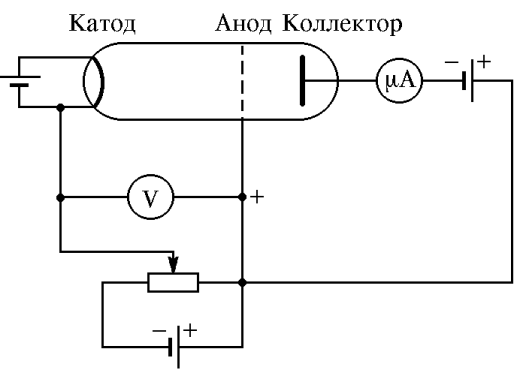
\includegraphics[width=\linewidth]{fig1}
	\caption{Cхема опыта Франка-Герца. Взято из \cite{lab}}
	\label{figure1}
\end{wrapfigure}

Одним из простых опытов, подтверждающих существование дискретных уровней энергии атомов, является эксперимент Франка и Герца. Схема опыта изображена на рис $\ref{figure1}$.

Разреженный одноатомный гелий заполняет трехэлектродную лампу. Электроны, испускаемые разогретым катодом, ускоряются в постоянном электрическом поле  созданным между катодом и сеткой. В зависимости от энергии электрона возможны упругие и неупругие столкновения с атомами гелия. При неупругих столкновениях электрон передает свою кинетическую энергию одному из атомных электронов, вызывая его переход на свободных энергетический уровень (возбуждение) или совсем отрывая его от атома (ионизация)

Третьим электродом лампы является коллектор. Ток коллектора, пропорциональный числу попадающих на него за секунду электронов, измеряется микроамперметром.

\begin{wrapfigure}{r}{0.3\linewidth} 
	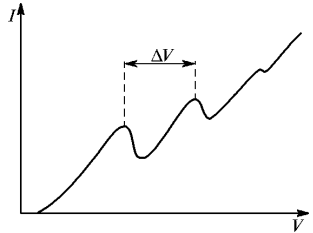
\includegraphics[width=\linewidth]{fig2}
	\caption{Зависимость тока коллектора от напряжения на аноде. Взято из \cite{lab}}
	\label{figure2}
\end{wrapfigure}

При увеличении потенциала на аноде ток в лампе вначале растет, однако, когда энергия электронов становится достаточной для возбуждения атомов, ток коллектор резко уменьшается. Это происходит потому, что при неупругих соударениях с атомами электроны почти полностью теряют свою энергию и не могут преодолеть задерживающий потенциал ($\approx$ 1В) между анодом и коллектором. При дальнейшем увеличении потенциала анода ток коллектора вновь возрастает: электроны, испытавшие неупругие столкновения, при дальнейшем движении к аноду успевают набрать энергию, достаточную для преодоления задерживающего потенциала.

Следующее замедление роста тока происходит в момент, когда часть электронов неупруго сталкивается с атомами два раза: первый раз посередине пути, второй у анода  и т.д. Таким образом, на кривой зависимости тока коллектора от напряжения анода имеется ряд максимумов и минимумов, отстоящие друго от друга на равные расстояние $\Delta V$; эти расстояние равны энергии первого возбужденного состояние (рис $\ref{figure1}$)

При тщательной постановке опыта можно увидеть и тонкую структуру кривой спада тока, содержащую ряд минимумов, возбуждению других уровней и ионизации атома гелия. Для этого нужны лампы специальной конструкции. В нашей постановке опыта эта тонкая структура не видна.

\newpage

\section*{Экспериментальная установка}

\begin{figure}[h]
    \centering
    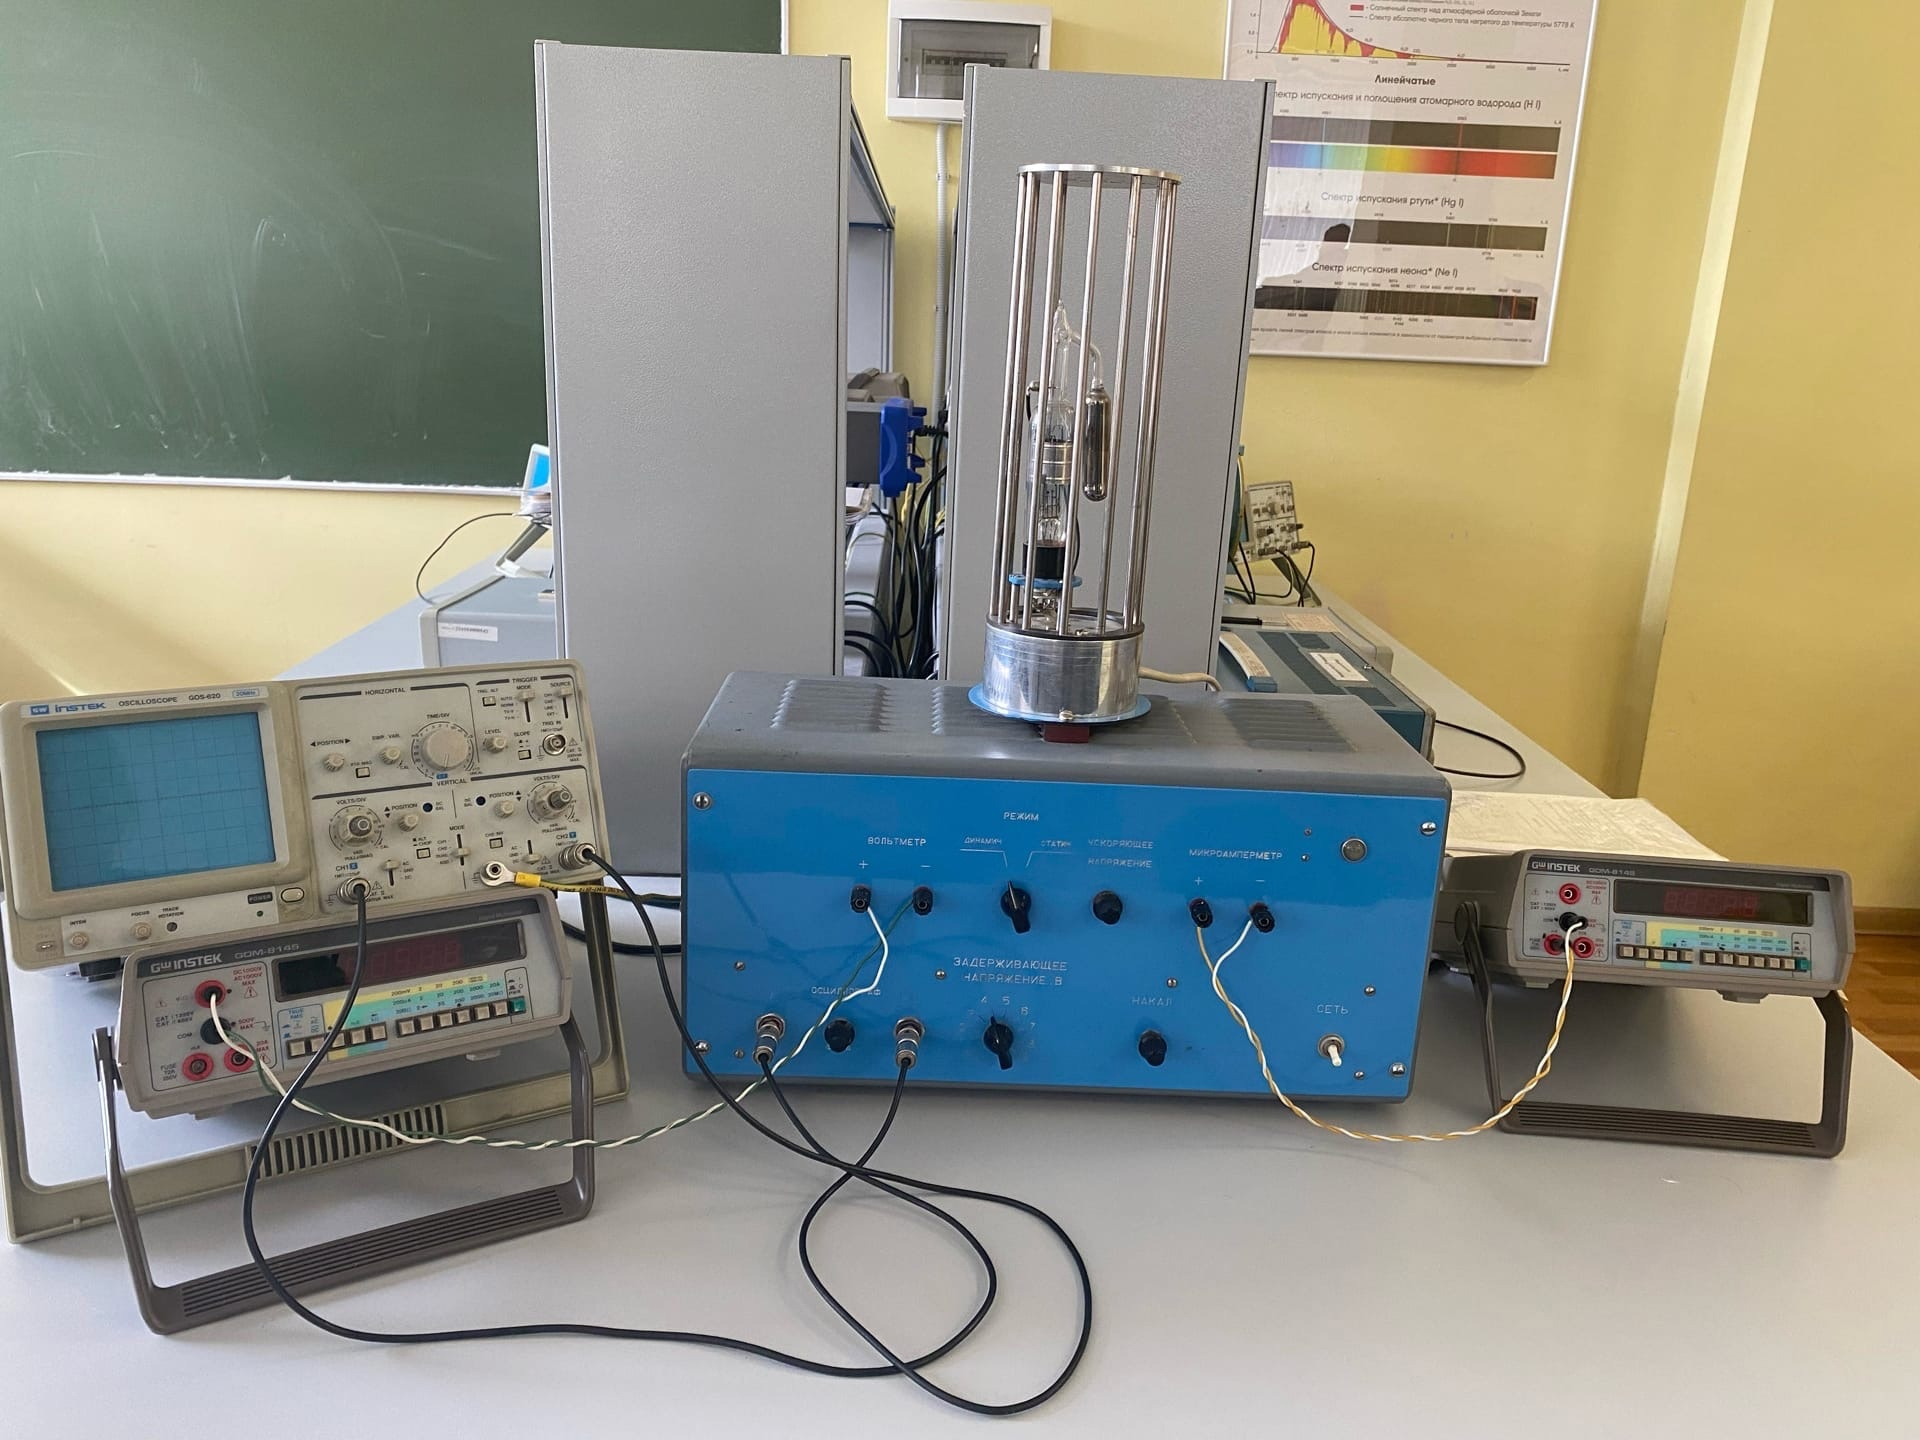
\includegraphics[width=15cm]{fig3}
    \caption{Схема экспериментальной установки}
    \label{fig:vac}
\end{figure}

\section*{Ход работы}

\subsubsection*{Получение вольт-амперной характеристики на экране осциллографа}

Поставим переключатель <<Режим>> в положение <<Динамич.>>, накал и ускоряющее напряжение установим на максимум.

Измерим расстояние между максимумами и между минимумами осциллограммы -- $\Delta V$ -- при разных значениях задерживающего напряжения ($U_з$). Полученные данные занесем в Таблицу \ref{table1} , учитывая что цена деления осциллографа -- 5 В/дел

\begin{table}[h!]
	\begin{center}
	\caption{Расстояния между минимумами и максимумами осциллограммы при различных запирающих напряжений}
	\label{table1}
	\begin{tabular}{|c|c|c|c|}
		\hline
		$U_з$, В & 4 & 6 & 8 \\ \hline
		$\Delta V_{max}$, В & 18,5 & 19 & {\color[HTML]{000000} 18} \\ \hline
		$\Delta V_{min}$, В & 20 & 20 & 21 \\ \hline
	\end{tabular}
	\end{center}
\end{table}

\newpage

Тогда среднее значение:

$$
	\overline {\Delta V} = 19,4 \pm 2,5 \ В,
$$

где погрешность рассчитывалась по формуле:
\begin{gather*}
	\sigma_{\Delta V} = 1 \ В - систематическая \ погрешность \ каждого \ измерения \\	
	%
	\sigma_{случ} = \sqrt{\frac{\sum \limits_{i=1}^{6} (\Delta V_i - \overline {\Delta V})^2 }{6 * 5}} \approx 0,5 \ В - случайная \ погрешность \\
	%	
	\sigma_{сист} = \sqrt{6 * \sigma_{\Delta V}^2} \approx 2,4 \ В \\
	%
	\sigma_{полн} = \sqrt{\sigma_{сист}^2 + \sigma_{случ}^2} \approx 2,5 \ В
\end{gather*}


\subsubsection*{Получение вольт-амперной характеристики в статическом режиме}

Поставим переключатель <<Режим>> в положение <<Статич.>>, установим максимальный накал и задерживающее напряжение на 4 В. Включим микроамперметр и вольтметр.

Плавно увеличивая ускоряющее напряжение -- $V_a$, снимем зависимость коллекторного тока от анодного напряжения $I_к = f(V_a)$ при разных значениях запирающего напряжения. Данные занесем в Таблицу $\ref{table2}$

\newpage

\begin{table}[h]
\centering
\caption{Зависимость коллекторного тока от анодного напряжения при различных  \\ значениях запирающего напряжения}
\label{table2}
\begin{minipage}{0.3\textwidth}
	\begin{tabular}{|cc|}
	\hline
	\multicolumn{2}{|c|}{\textbf{$U_з$   = 4 В}} \\ \hline
	\multicolumn{1}{|c|}{\textbf{$U_a$, В}} & \textbf{I, мА} \\ \hline
	\multicolumn{1}{|c|}{21,11} & 0,252 \\ \hline
	\multicolumn{1}{|c|}{21,90} & 0,249 \\ \hline
	\multicolumn{1}{|c|}{22,33} & 0,243 \\ \hline
	\multicolumn{1}{|c|}{23,02} & 0,211 \\ \hline
	\multicolumn{1}{|c|}{23,70} & 0,194 \\ \hline
	\multicolumn{1}{|c|}{24,05} & 0,198 \\ \hline
	\multicolumn{1}{|c|}{24,61} & 0,205 \\ \hline
	\multicolumn{1}{|c|}{25,11} & 0,216 \\ \hline
	\multicolumn{1}{|c|}{25,67} & 0,227 \\ \hline
	\multicolumn{1}{|c|}{26,07} & 0,235 \\ \hline
	\multicolumn{1}{|c|}{27,10} & 0,253 \\ \hline
	\multicolumn{1}{|c|}{27,94} & 0,268 \\ \hline
	\multicolumn{1}{|c|}{28,66} & 0,288 \\ \hline
	\multicolumn{1}{|c|}{29,60} & 0,308 \\ \hline
	\multicolumn{1}{|c|}{30,56} & 0,327 \\ \hline
	\multicolumn{1}{|c|}{33,18} & 0,375 \\ \hline
	\multicolumn{1}{|c|}{36,14} & 0,412 \\ \hline
	\multicolumn{1}{|c|}{38,10} & 0,414 \\ \hline
	\multicolumn{1}{|c|}{39,07} & 0,411 \\ \hline
	\multicolumn{1}{|c|}{40,18} & 0,401 \\ \hline
	\multicolumn{1}{|c|}{41,20} & 0,392 \\ \hline
	\multicolumn{1}{|c|}{42,06} & 0,390 \\ \hline
	\multicolumn{1}{|c|}{43,16} & 0,388 \\ \hline
	\multicolumn{1}{|c|}{43,98} & 0,389 \\ \hline
	\multicolumn{1}{|c|}{44,47} & 0,391 \\ \hline
	\end{tabular}
\end{minipage}
\begin{minipage}{0.3\textwidth}
\begin{tabular}{|cc|}
\hline
\multicolumn{2}{|c|}{\textbf{$U_з$   = 6 В}} \\ \hline
\multicolumn{1}{|c|}{\textbf{$U_a$, В}} & \textbf{I, мА} \\ \hline
\multicolumn{1}{|c|}{36,24} & 0,361 \\ \hline
\multicolumn{1}{|c|}{37,20} & 0,364 \\ \hline
\multicolumn{1}{|c|}{38,20} & 0,366 \\ \hline
\multicolumn{1}{|c|}{39,09} & 0,362 \\ \hline
\multicolumn{1}{|c|}{39,59} & 0,359 \\ \hline
\multicolumn{1}{|c|}{40,50} & 0,350 \\ \hline
\multicolumn{1}{|c|}{41,23} & 0,343 \\ \hline
\multicolumn{1}{|c|}{42,00} & 0,337 \\ \hline
\multicolumn{1}{|c|}{42,46} & 0,335 \\ \hline
\multicolumn{1}{|c|}{44,06} & 0,324 \\ \hline
\multicolumn{1}{|c|}{44,58} & 0,322 \\ \hline
\multicolumn{1}{|c|}{45,18} & 0,321 \\ \hline
\multicolumn{1}{|c|}{45,66} & 0,319 \\ \hline
\multicolumn{1}{|c|}{46,22} & 0,318 \\ \hline
\multicolumn{1}{|c|}{47,00} & 0,318 \\ \hline
\multicolumn{1}{|c|}{47,38} & 0,319 \\ \hline
\multicolumn{1}{|c|}{48,35} & 0,323 \\ \hline
\multicolumn{1}{|c|}{49,10} & 0,326 \\ \hline
\end{tabular}
\end{minipage}
\begin{minipage}{0.3\textwidth}
\begin{tabular}{|ll|}
\hline
\multicolumn{2}{|c|}{\textbf{$U_з$ = 8 В}} \\ \hline
\multicolumn{1}{|c|}{\textbf{$U_a$, В}} & \multicolumn{1}{c|}{\textbf{I, мА}} \\ \hline
\multicolumn{1}{|l|}{3,00} & 0,001 \\ \hline
\multicolumn{1}{|l|}{7,24} & 0,054 \\ \hline
\multicolumn{1}{|l|}{10,06} & 0,109 \\ \hline
\multicolumn{1}{|l|}{15,16} & 0,195 \\ \hline
\multicolumn{1}{|l|}{18,06} & 0,236 \\ \hline
\multicolumn{1}{|l|}{20,24} & 0,259 \\ \hline
\multicolumn{1}{|l|}{20,90} & 0,261 \\ \hline
\multicolumn{1}{|l|}{21,94} & 0,260 \\ \hline
\multicolumn{1}{|l|}{22,39} & 0,257 \\ \hline
\multicolumn{1}{|l|}{23,13} & 0,247 \\ \hline
\multicolumn{1}{|l|}{23,95} & 0,217 \\ \hline
\multicolumn{1}{|l|}{25,24} & 0,094 \\ \hline
\multicolumn{1}{|l|}{26,31} & 0,094 \\ \hline
\multicolumn{1}{|l|}{26,69} & 0,096 \\ \hline
\multicolumn{1}{|l|}{27,43} & 0,105 \\ \hline
\multicolumn{1}{|l|}{28,05} & 0,116 \\ \hline
\multicolumn{1}{|l|}{29,93} & 0,165 \\ \hline
\multicolumn{1}{|l|}{32,20} & 0,218 \\ \hline
\multicolumn{1}{|l|}{34,21} & 0,261 \\ \hline
\multicolumn{1}{|l|}{36,22} & 0,291 \\ \hline
\multicolumn{1}{|l|}{38,02} & 0,296 \\ \hline
\multicolumn{1}{|l|}{38,80} & 0,300 \\ \hline
\multicolumn{1}{|l|}{39,86} & 0,293 \\ \hline
\multicolumn{1}{|l|}{40,65} & 0,286 \\ \hline
\multicolumn{1}{|l|}{41,89} & 0,277 \\ \hline
\multicolumn{1}{|l|}{43,58} & 0,263 \\ \hline
\multicolumn{1}{|l|}{44,57} & 0,254 \\ \hline
\multicolumn{1}{|l|}{46,09} & 0,243 \\ \hline
\multicolumn{1}{|l|}{48,28} & 0,235 \\ \hline
\multicolumn{1}{|l|}{49,12} & 0,235 \\ \hline
\multicolumn{1}{|l|}{50,02} & 0,238 \\ \hline
\end{tabular}
\end{minipage}
\end{table}	

По полученным данным построим графики, учитывая что $\sigma_{U_a} = 0,01 \ В$, $\sigma_{I} = 0,05 \ мА $.

\newpage

\begin{figure}[h!]
	\centering
	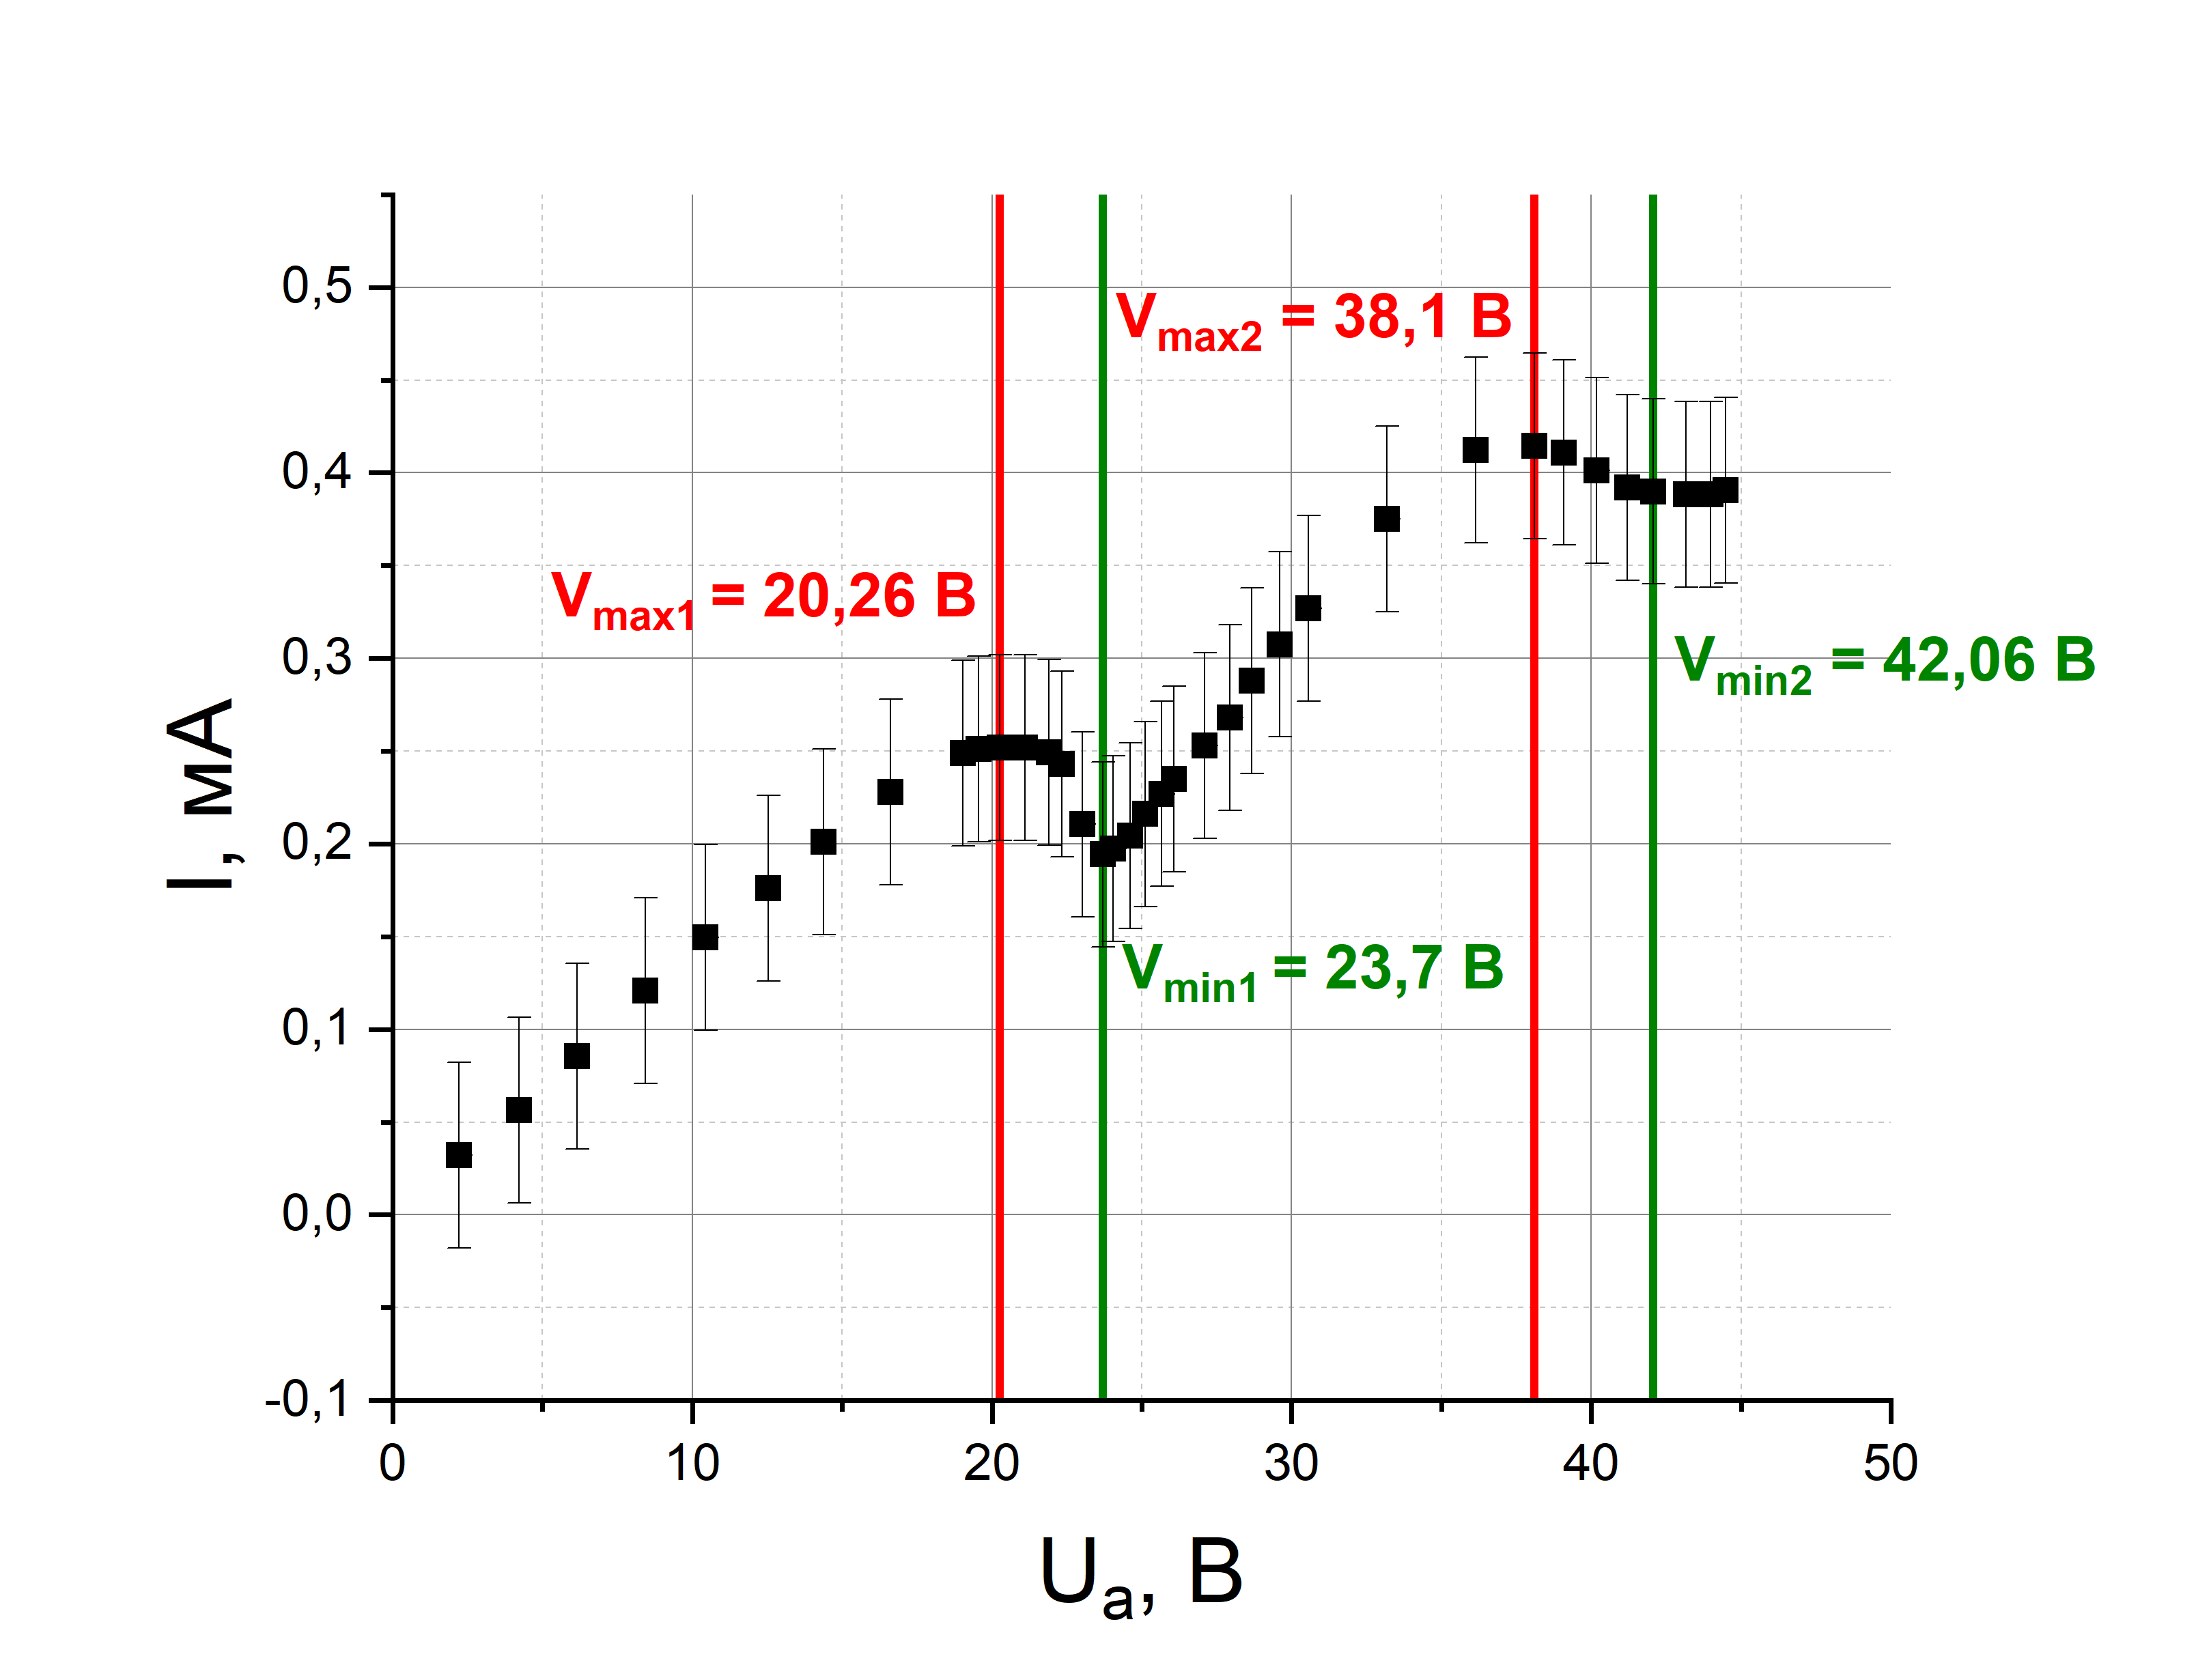
\includegraphics[scale=0.5]{graph1}
	\caption{Зависимость $I_к = f(V_a)$ в статическом режиме при $U_з$ = 4 В}
	\label{graph1}
\end{figure}

\begin{figure}[h!]
	\centering
	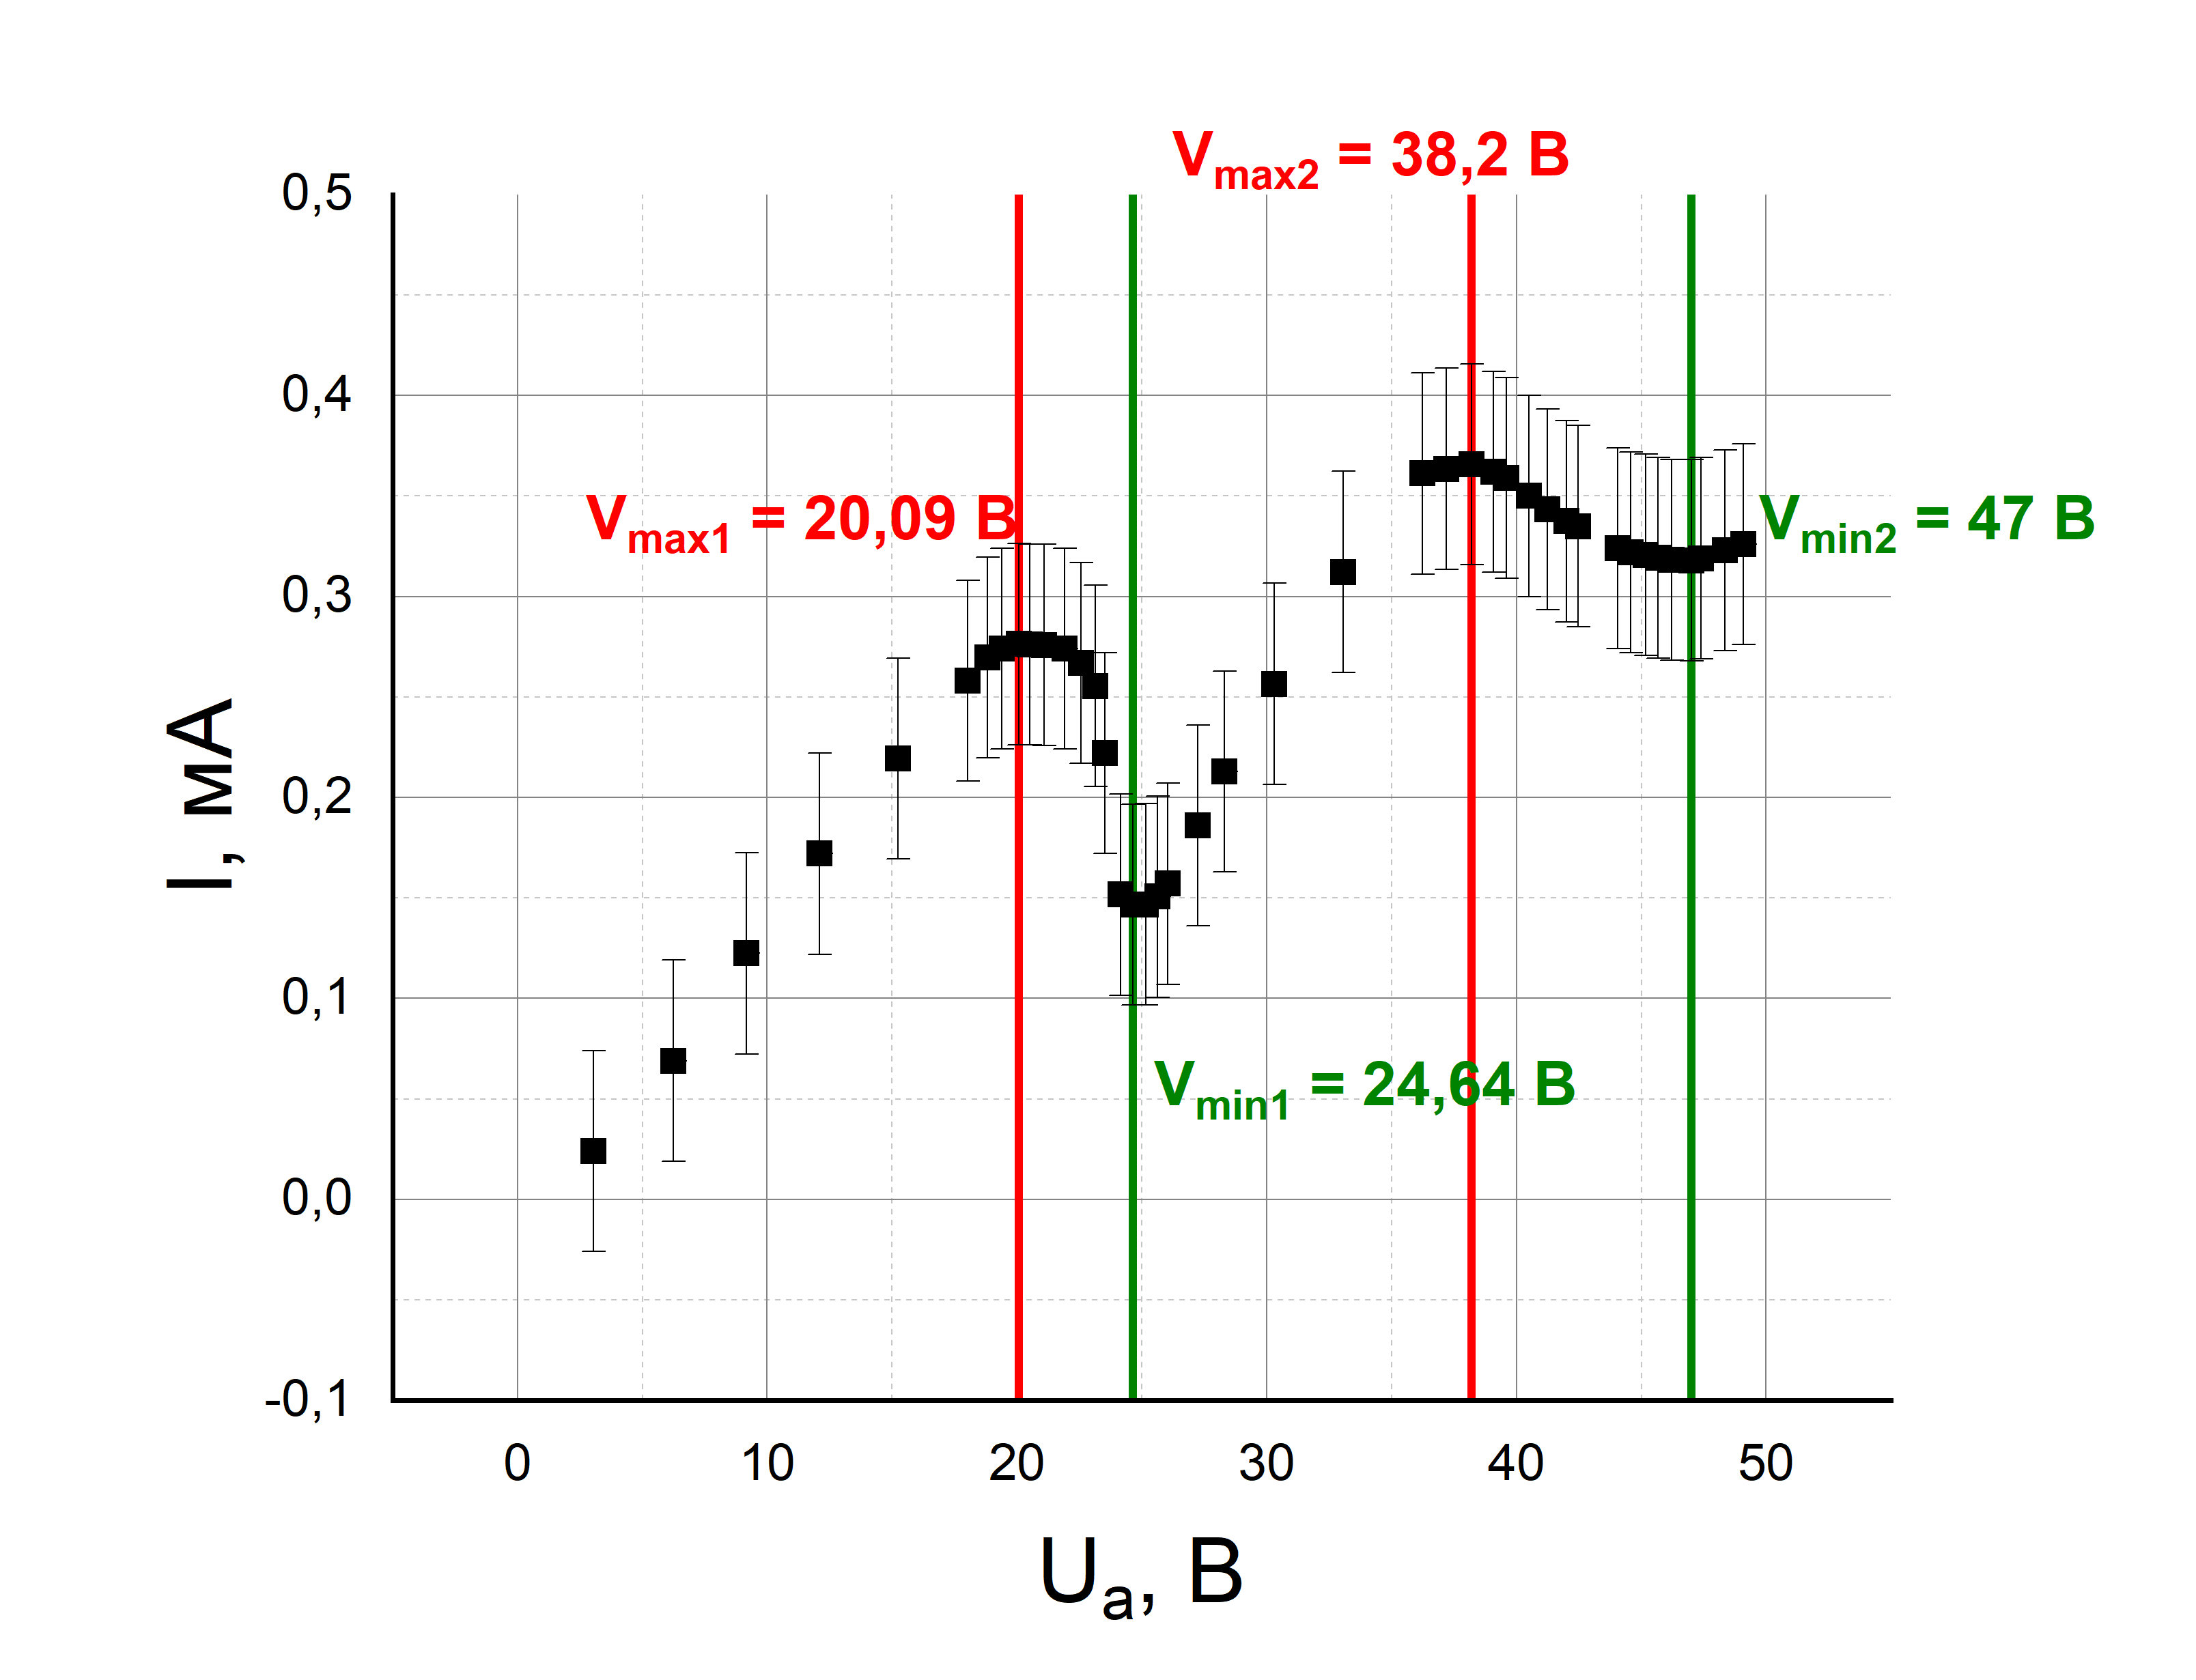
\includegraphics[scale=0.5]{graph2}
	\caption{Зависимость $I_к = f(V_a)$ в статическом режиме при $U_з$ = 6 В}
	\label{graph2}
\end{figure}

\newpage

\begin{figure}[h!]
	\centering
	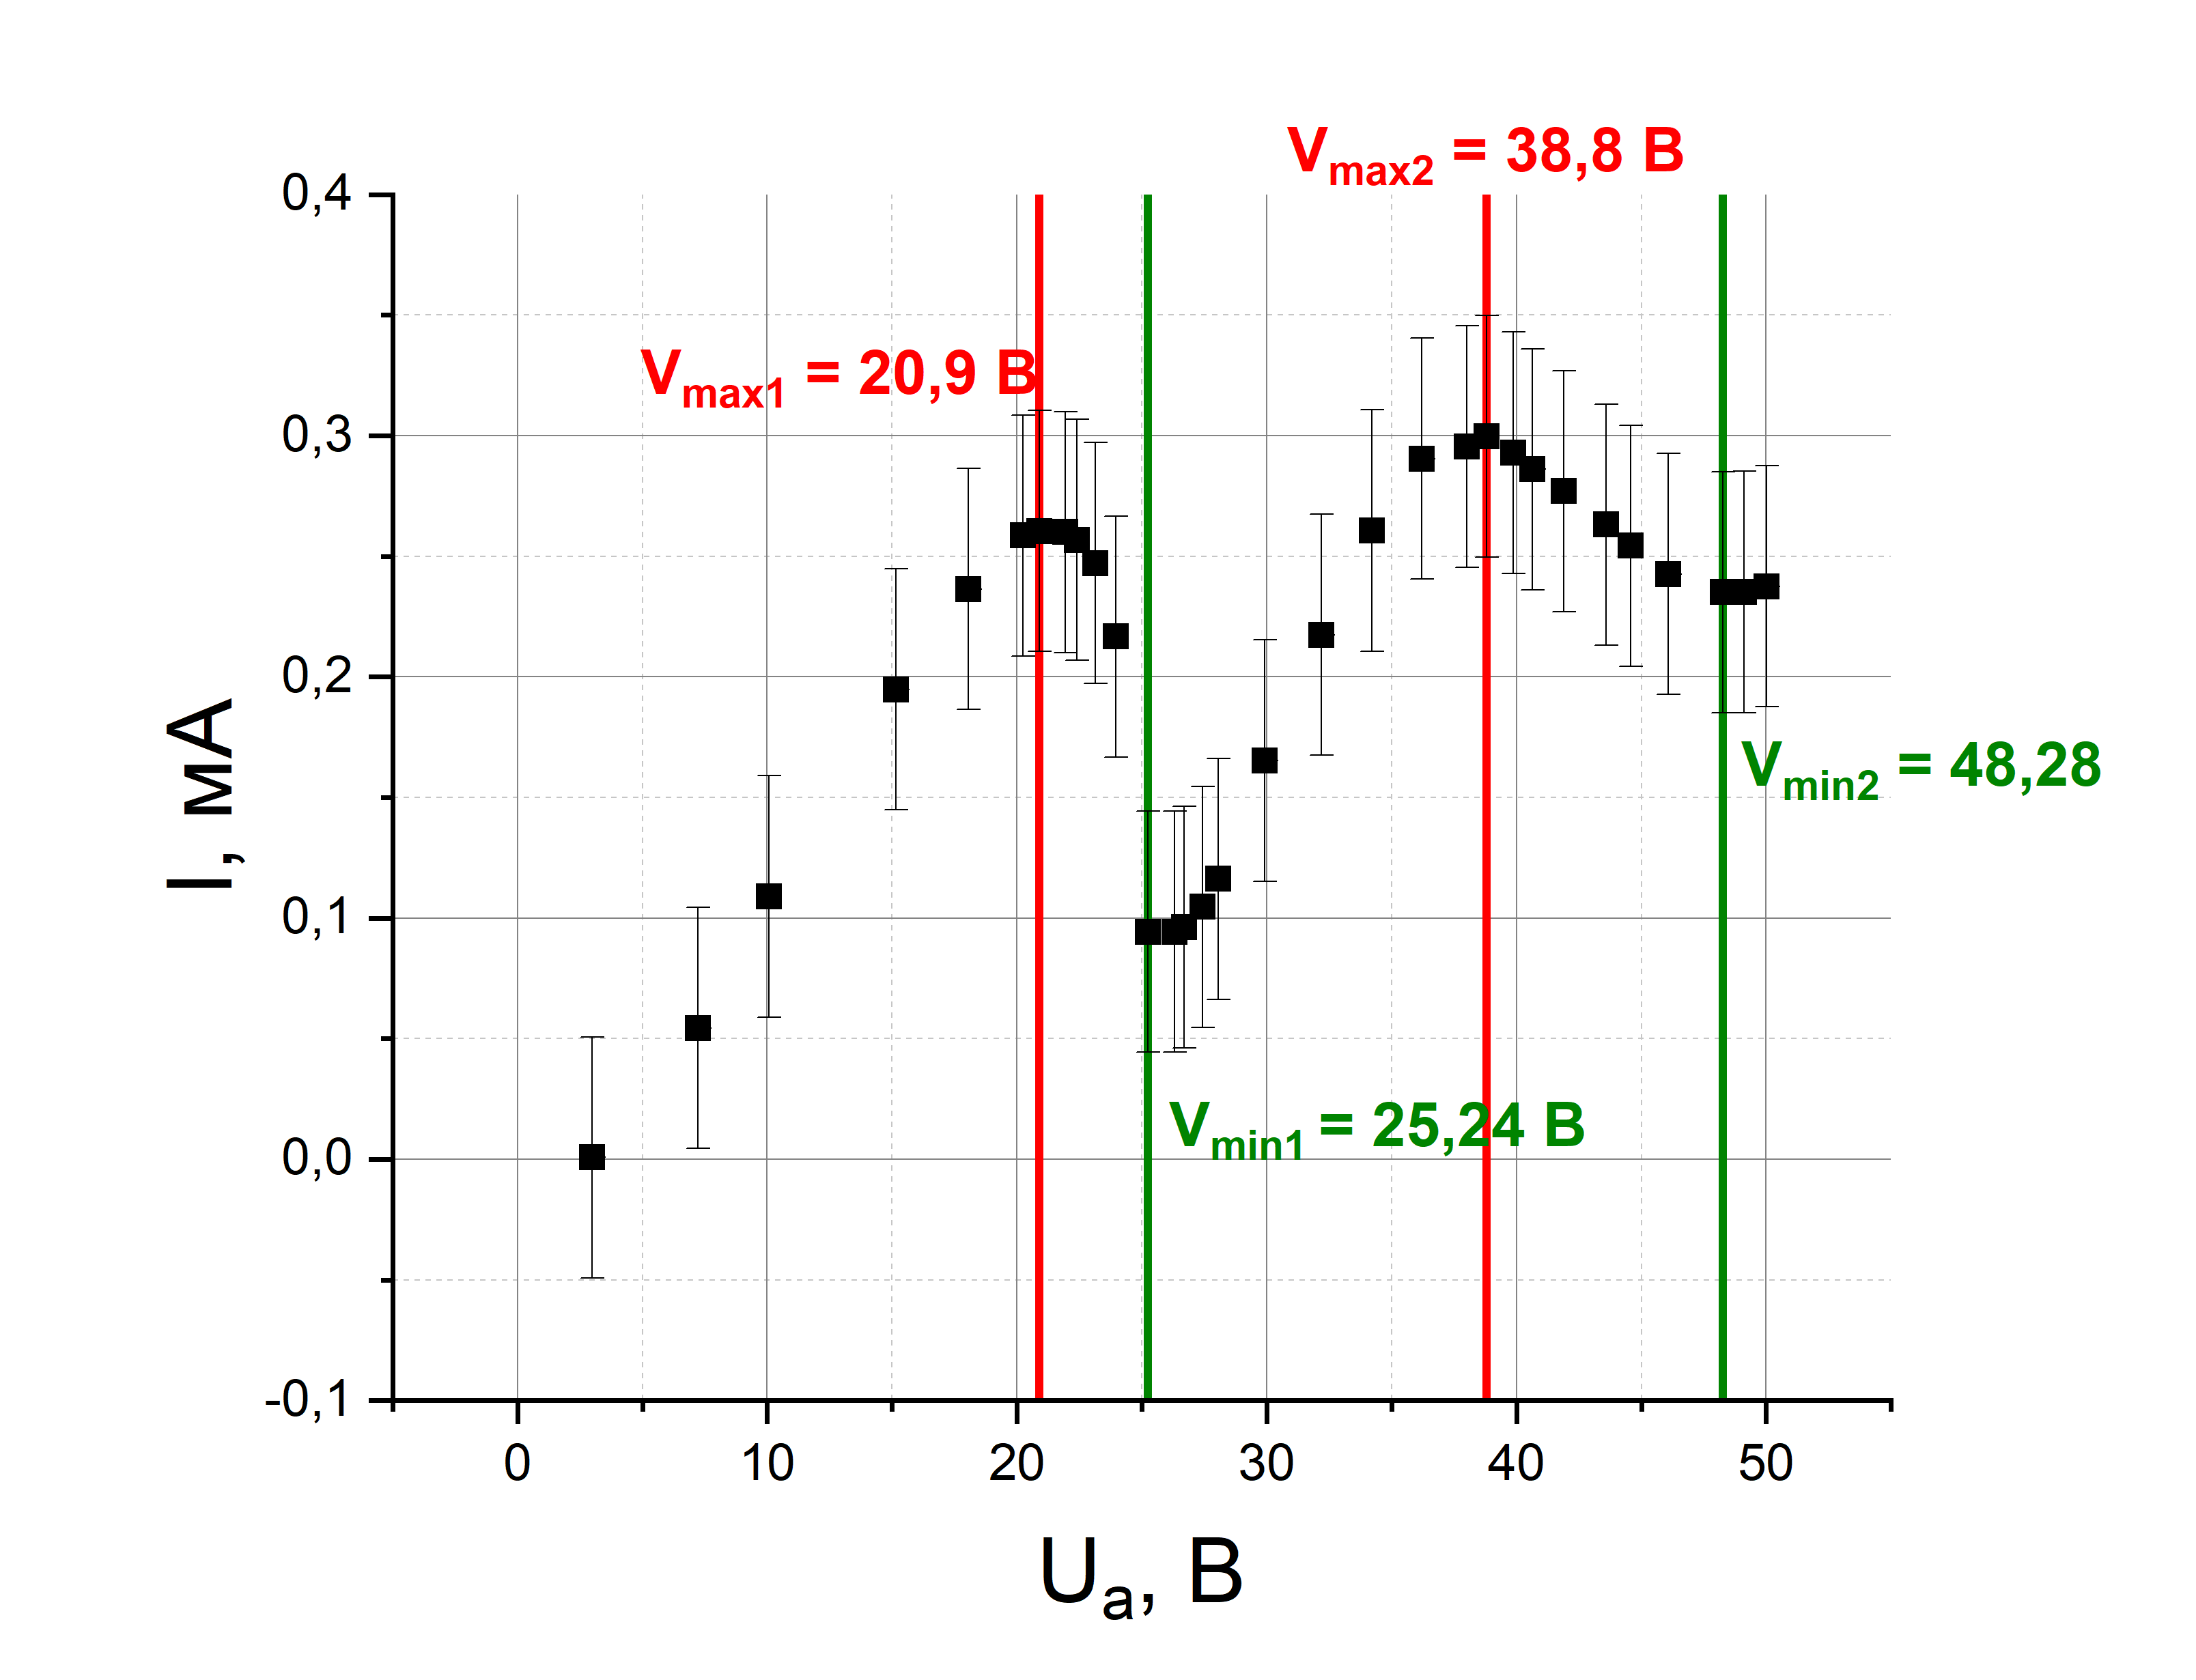
\includegraphics[scale=0.5]{graph3}
	\caption{Зависимость $I_к = f(V_a)$ в статическом режиме при $U_з$ = 8 В}
	\label{graph3}
\end{figure}

Рассчитаем разницу $\Delta V$ значений анодного напряжения между последовательными максимумами и минимумами графика при различных значениях запирающего напряжения. Данные занесем в Таблицу  $\ref{table3}$

\begin{table}[h]
	\centering
	\caption{Разница значений анодного напряжения между последовательными максимумами и минимумами зависимости $I_к = f(U_a)$ при различных значениях запирающего напряжения}
	\label{table3}
	\begin{tabular}{|c|c|c|c|}
	\hline
	\textbf{$U_з$, В} & 4 & 6 & 8 \\ \hline
	\textbf{$\Delta V_{max}$, В} & 17,84 & 18,11 & 17,90 \\ \hline
	\textbf{$\Delta V_{min}$, В} & 18,36 & 22,36 & 23,04 \\ \hline
	\end{tabular}
\end{table}

Тогда среднее значение:

$$
	\overline {\Delta V} = 19,6 \pm 1,0 \ В,
$$

где погрешность рассчитывалась по формуле:
\begin{gather*}
	\sigma_{\Delta V} = 0,01 \ В - систематическая \ погрешность \ каждого \ измерения \\	
	%
	\sigma_{случ} = \sqrt{\frac{\sum \limits_{i=1}^{6} (\Delta V_i - \overline {\Delta V})^2 }{6 * 5}} \approx 1 \ В - случайная \ погрешность \\
	%	
	\sigma_{сист} = \sqrt{6 * \sigma_{\Delta V}^2} \approx 0,02 \ В \\
	%
	\sigma_{полн} = \sqrt{\sigma_{сист}^2 + \sigma_{случ}^2} \approx 1 \ В
\end{gather*}

\newpage

\section*{Выводы}

1.В ходе работы были получены значения для первого возбужденного состояния атома гелия двумя способами -- динамическим и статическим.
$$
	\Delta V_{статич} = 19,4 \pm 2,5 \ эВ 
$$
$$
	\Delta V_{динамич} = 19,6 \pm 1 \ эВ 
$$
$$
	\Delta V_{теор} = 20,96 \ эВ  
$$


Значение, полученное статическим методом, совпадает с теоретическим, в пределах погрешности. 

Значение, полученное динамическим методом, отличается от теоретического на 2 \%. Данное расхождение может быть связано с тем, что систематическая погрешность вольтметра составляет более 0,01 В.

2. Таким образом, в нашем случае статический метод является более точным.

\begin{thebibliography}{2}
	\bibitem{lab} \emph{Лабораторный практикум по общей физике. Квантовая физика} под ред. Ю. М. Ципенюка
	\bibitem{opisanie} \emph{Дополнительное описание. Опыт Франка-Герца}
\end{thebibliography}

\end{document}